\section*{Úvod}
\addcontentsline{toc}{section}{Úvod} 
\indent\indent Cílem mé práce bylo navrhnout a realizovat SDR přijímač pro pásmo krátkých vln. Toto téma spojuje mikroprocesorovou a číslicovou techniku s radioelektronikou, kterou jsem si chtěl osahat. V úvodu bych chtěl dále vysvětlit, co se skrývá za zkratkou SDR.

Zkratka SDR znamená Software Defined Radio (v překladu Softwarově Definované Rádio). Jedná se o další vývojovou etapu rádiových přijímačů a vysílačů. Klasická analogová rádia se postupně vyvíjela od jednoduchých krystalových přijímačů s přímým zesílením, přes přímosměšující tranzistorové přijímače až k velmi složitým přijímačům typu superheterodyn s možnostmi přepínání nejrůznějších demodulací a velkým rozsahem přijímaných pásem. Tyto přijímače ale začínaly být tak složité, že se k napěťovým signálům nesoucím informace při jejich zpracování přičítal šum jednotlivých bloků. Tento šum pak výrazně zhoršoval kvalitu přijímaného signálu. SDR je moderní technologie, která se snaží tyto nežádoucí vlivy hardwarových komponentů omezit. Ideální SDR přijímač se skládá jen z antény analogově digitálního převodníku a digitálního obvodu, který signál demoduluje. Díky tomu se k přijímané informaci přidává jen minimální chyba při digitalizaci signálu. Tato technologie tedy posouvá zařízení pro rádiový přenos o světelné roky dál, jelikož je s jejich pomocí možné přenášet v podstatě libovolně modulovaný signál, a tím pak přenášet komprimované informace, nebo vytvářet nové digitální modulace. Obrovskou výhodou SDR přijímačů a vysílačů je jejich neustálé vylepšování bez nutnosti jakkoliv měnit hardware přijímače.
\begin{figure}[H]
	\centering
	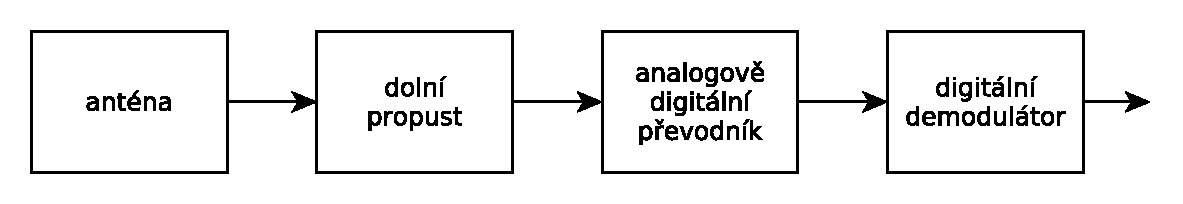
\includegraphics[width=170mm]{img/i_sdr.pdf}
	\caption{blokové schéma ideálního SDR přijímače}    		
\end{figure}

\clearpage
		
	
  		
  		